\documentclass[letterpaper, 12pt]{article}
\usepackage[letterpaper, top=2.5cm, bottom=2.5cm, left=3cm, right=3cm]{geometry} %margenes
\usepackage[utf8]{inputenc} %manejo de caracteres especiales
\usepackage[spanish]{babel} %manejo de encabezados de inglés a español
\usepackage{fancyhdr} %formato de los encabezados de página
\usepackage{ragged2e} %alineado real justficado
\usepackage{graphicx} %manejo de imagenes
\usepackage{amsmath} %manejo de notación matemática
\usepackage{mathtools} %manejo de notación matemática
\usepackage{blindtext} %texto de relleno
\usepackage{float}
\usepackage[backend=biber]{biblatex}\addbibresource{referencias.bib} %manejo de bibliografía (BORRAR SI NO ES NECESARIO)

\pagestyle{empty}
\fancyhf{}
\rfoot{\thepage}

\nocite{*}

\begin{document}
    
    %PORTADA
    \begin{titlepage}
        \begin{figure}[ht]
            \centering
            
\includegraphics[width=15cm]{logosITT.png}
        \end{figure}
        \centering
        {\scshape\LARGE Tecnológico Nacional de México\\Instituto Tecnológico de Tijuana\par}
        \vspace{1cm}
        {\scshape\Large Graficación\par}
        \vspace{1cm}
        {\scshape\Large Unidad 1\par}
        \vspace{1.5cm}
        {\huge\bfseries Tarea 1\par}
        \vspace{2cm}
        {\Large\itshape C. Abraham Jhared Flores Azcona\\\#: 19211640\par}
        \vfill
        Profesor: \par
        Dra. Martha Elena Pulido
        
        \vfill

        {\large 26 de agosto de 2021}
    \end{titlepage}

    \newpage
    \begin{justify}
        \thispagestyle{empty}
        En esta breve investigación se desarrollan las contribuciones importantes de tres figuras prominentes y/o relevantes al área de la graficación.
        \section*{Tony DeRose}
        Actualmente el Científico Senior en los Estudios Animados Pixar. Recibió una licenciatura en Física en 1981 de la Universidad de California, Davis;
        en 1985 él recibe un Doctorado en Ciencias Computacionales de la Universidad de California, Berkeley. Recibió el premio del Investigador Presidencial Joven por la
        Asociación Nacional de Ciencia de los Estados Unidos en 1989.
        \\\newline
        Sus investigaciones se enfocan en los modelos matemáticos
        para el modelado de superficies, acomodado de datos, y recientemente, en el uso de técnicas multiresolución. Proyectos recientes incluyen la adquisición de objetos de 
        los datos de longitud de láseres y métodos multiresolución/wavelet para gráficos computacionales de alto rendimiento, y métodos para la animación de personajes humanos.
        \begin{figure}[H]
            \centering
            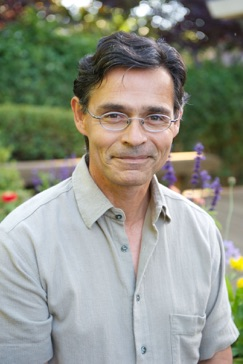
\includegraphics[width=5cm,height=8cm]{tony.jpeg}
            \caption{Foto del Dr. Tony DeRose.} 
        \end{figure}
        \section*{Rene Descártes}
        Filósofo prominente en distintas áreas del conocimiento. Desarrolló la geometría analítica, particularmente los sistemas de coordenadas que (en honor a él) llevan su nombre, por ende los planos cartesianos. Estos planos nos proveen una fundación
        para describir la posición y la forma de los objetos en el espacio que es un aspecto fundamental en la graficación por computadora.
        \begin{figure}[H]
            \centering
            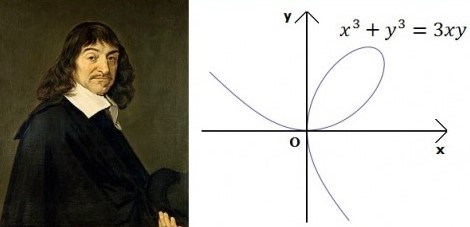
\includegraphics[width=10cm,height=6cm]{descartes.jpg}
            \caption{Imágen  de René Descartes junto a un plano cartesiano con una gráfica.}
        \end{figure}
        \section*{Pierre Bézier}
        Ingenierio francés. Fue uno de los fundadores de los campos de modelado de sólidos, modelado geométrico y físico así como en el campo de curvas representativas, especialmente en diseño apoyado por computadora y sistemas de manufacturas.
        Como ingeniero de Renault, logró popularizar y patentar las curvas de Bézier al usarlas para diseñar cuerpos de automóviles. A pesar de esas curvas llevan su nombre, estas fueron desarrolladas primeramente por Paul de Casteljau en 1959. Bézier
        desarrolló la notación que consiste en nodos con manijas de control añadidas, con las cuales las curves son representadas en software de computadoras.
        \begin{figure}[H]
            \centering
            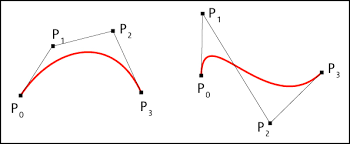
\includegraphics[width=8cm,height=6cm]{bezier.png}
            \caption{Ejemplos de dos curvas de Bézier cúbicas. El grado de la curva es el totál de puntos menos uno.}
        \end{figure}
        \section*{Conclusiones}
        Estas tres personalidades han aportado contribuciones en distitnos aspectos de la graficación, desde el lenguaje matemático, hasta complejidades antes no exploradas. Por ello es relevante revisar sus avances para apreciar la facilidad que nos han dado para
        el estudio, comprensió y aplicación de la graficación.
    \end{justify}

    \newpage
        \thispagestyle{empty}
        \printbibliography  
\end{document}